\section{Planes}

If $(x,y,z)$ is a point on the plane, then given $\vec{P}_0=(x_0,y_0,z_0)$, $(x-x_0,y-y_0,z-z_0)$ is a vector on the plane perpendicular to $\vec{n}$, the
normal vector. Thus, $(A,B,C)\cdot(x-x_0,y-y_0,z-z_0)=0$ where $A,B,C$ are vector coordinates of $\vec{n}$. With expansion:

\begin{align*}
    A(x-x_0)+B(y-y_0)+C(z-z_0)&=0\\
    Ax+By+Cz=Ax_0+By_0+Cz_0&=0\\
    Ax+By+Cz=\vec{n}\cdot \vec{P}_0
\end{align*}

Note that $(A,B,C)$ form coordinates of $\vec{n}$.

To find a plane containing 3 points $\vec{v}_1,\vec{v}_2,\vec{v}_3$, compute, for example $\vec{c}_1=\vec{v}_3-\vec{v}_1$ and $\vec{c}_2=\vec{v}_2-\vec{v}_1$.
This finds 2 vectors in the plane. Then compute $\vec{c}_1\times \vec{c}_2=\vec{n}$. \newline

\noindent
The trace of a plane is the intersection of a plane $\mathcal{P}$ with $xy$, $xz$, or $yz$ coordinate planes. Can be found by setting respective variable to 0.
\subsection{Cross-product rules and identities}

Overview
\begin{itemize}
    \item $||\vec{a}\times \vec{b}||=||\vec{a}||||\vec{b}||\sin\theta$
    \item $\vec{a},\vec{b}\perp \vec{a}\times \vec{b}$
\end{itemize}

Algebraic
\begin{itemize}
    \item $\vec{a}\times \vec{b}=\vec{0}$
    \item $\vec{a}\times \vec{b}=-\vec{b}\times \vec{a}$
    \item Distributive properties hold -- preserve direction however
    \item $(\alpha \vec{a})\times \vec{b}=\alpha(\vec{a}\times \vec{b})$
\end{itemize}

\section{Graphs}

\subsection{Multivariable functions}

Function of $n$-variables is real-valued function with $f(x_1,\cdots,x_n)$ with domain $\mathcal{D}$
being a set of $n$-tuples $(x_1,\cdots,x_n)$ in $\R^n$, or where $f$ is defined.
Range of $f$ is all values $f(x_1,\cdots,x_n)$ for $(x_1,\cdots,x_n)$ in the domain.

\subsection{Graphing multivariable functions}

Traces are 2D curves obtained by intersection with planes parallel to coordinate plane.
\begin{itemize}
    \item Horizontal trace at height $c$ -- intersection of graph with plane $z=c$, so points $(x,y,c)$ such that $f(x,y)=c$
    \item Vertical trace in plane $x=a$ -- intersection of graph with vertical plane $x=a$ for all points $(a,y,f(a,y))$
    \item Vertical trace in plane $y=b$ -- intersection of graph with vertical plane $y=b$ for all points $(x,b,f(x,b))$
\end{itemize}

\begin{center}
    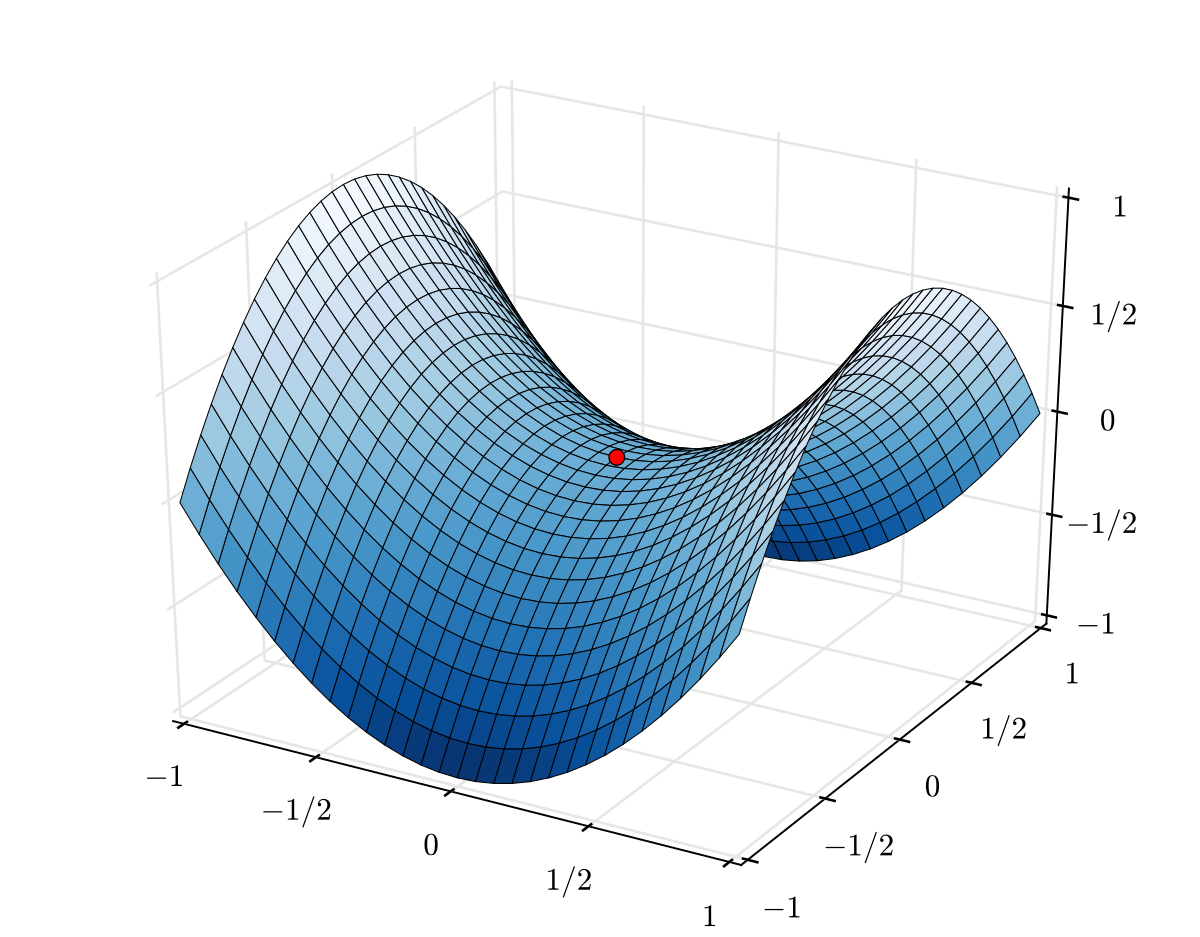
\includegraphics[scale=0.15]{saddle-plot.png}
\end{center}

Saddle surface general form is $f(x,y)=x^2-y^2$. The horizontal traces are hyperbolas of the form $c=x^2-y^2$.
Vertical traces are parabolas, as either $x,y$ set to 0.\newline

\noindent
Linear functions in 2 variables are of the form $f(x,y)=mx+ny+r|m,n,r\in \R$.

\subsection{Contour maps and level curves}

\begin{center}
    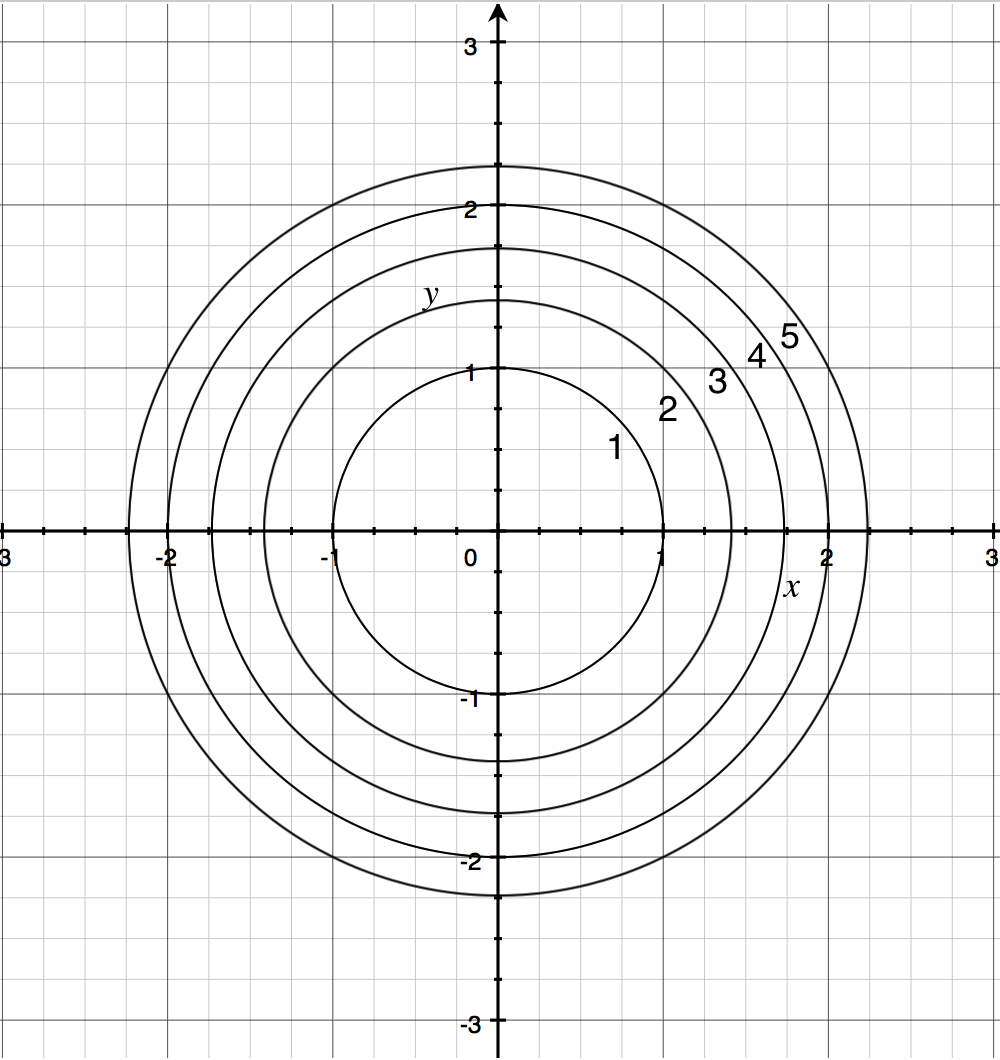
\includegraphics[scale=0.15]{contour-map.png}
\end{center}

Can specify a contour interval for each $z=c$ value. Is a 2D representation of
level curves of $f(x,y)$ at an interval. Going along level curve means change in altitude is
0. Altitude has change of $\pm m$ (contour interval) when going up/down contour levels.\newline